\documentclass[11pt,a4paper,english,oneside]{book}
\usepackage{etex} %Because of many packages --> Extended TeX.
\usepackage[left=1in, right=1in]{geometry} %Helps to structure the paper layout.
\usepackage[Lenny]{fncychap} %Design of the thesis.
\usepackage[utf8]{inputenc} %Due to vowels.
\usepackage{babel} %Define the language style.
\usepackage{dsfont} %Nice style for the indicator function.
\usepackage{fancyhdr} %To customize the headers and footers.
\usepackage{booktabs} %In case you need \cmidrule or \addlinespace in tables.
\usepackage[hang,bottom,stable,multiple]{footmisc} %Style of footnotes.
\usepackage{appendix} %For the \appendixpage command.
%Load some mathematical packages.
\usepackage{amsmath}
\usepackage{amsfonts}
\usepackage{amsmath}
\usepackage{amssymb}
\usepackage{mathtools}
%\usepackage[sort,round]{natbib} %For the bibliography.
\usepackage[natbibapa]{apacite} %for citing and bibliography, by Corinne
\usepackage{etoolbox} %To remove the page number on \appendixpage.
\usepackage{amsthm} %For theorems, definitions etc.
\usepackage{thmtools} %For theorems, definitions etc.
\usepackage{setspace} %Use double spacing.
\usepackage{lipsum} %For the \lipsum command to generate a text.
\usepackage{datetime} %For the specification of the date.
%\usepackage{tocloft} %The ToC, LoF and LoT each appear not necessarily on a new page.
\usepackage{graphicx,listings, xcolor, colortbl, textcomp} %For the graphics, listings etc.
\usepackage{mcode} %To implement a Matlab code.
\usepackage[margin=10pt, font=small, labelfont=bf, labelsep=endash]{caption} %Customize the captions.
\usepackage{chngcntr} %To use counterwithout.
\usepackage{epstopdf} %For inserting .eps files into the document.
\usepackage{hyperref} %Must be loaded at the end.
\usepackage{xparse} %Load for \NewDocumentCommand command.
\usepackage{cleveref} %For the command \cref, load after hyperref.
\usepackage{arydshln} %Due to the capability to draw horizontal/vertical dash-lines.
\usepackage{array,hhline} %To create tables and matrices.
\usepackage{rotating} %To rotate a table.
\usepackage{tabularx} %An extended version of tabular.

%Setup of the reference links.
\hypersetup{
     colorlinks=false,
     linkcolor=blue,
     citecolor=blue,
     filecolor=magenta,
     urlcolor=blue}

%Define some reasonable margins.
%\setlength{\textwidth}{6.6in}
\setlength{\textheight}{9.3in}
\setlength{\topmargin}{-0.1in}
%\setlength{\oddsidemargin}{0in}
\setlength{\parskip}{1mm}

\bibliographystyle{apacite} %Reference style.
\allowdisplaybreaks[1] %Page breaks of equations are allowed, but avoided if possible. 2-4 more relaxed.

%New command for the logo.
\newcommand*{\plogo}{
\includegraphics[scale=0.7]{Images/HSG_logo}}

%New command for the differential d to have an ordinary d.
\makeatletter
  \newcommand{\ud}{\mathrm{d}}
\makeatother

%Remove page number on \appendixpage. Use the package 'etoolbox'.
\makeatletter
\patchcmd{\@chap@pppage}{\thispagestyle{plain}}{\thispagestyle{empty}}{}{}
\makeatother

%Declare Definitions, Theorems etc.
%%%%%%%%%%%%%%%%%%%%%%%%%%%%%%%%%%%%%%%%%%%%%%%%%%%%%%%%%%%%%%%%%%%%%%%%%%%%%%%%%%%%%%%%%%%%%%%%%%%%%%%%%%%%%%%%%%%
\declaretheorem[style=definition,qed=$\blacktriangleleft$, numberwithin=chapter]{remark} %additional options; numberwithin=,..., see 'Thmtools' Users’ Guide
\declaretheorem[style=definition,qed=$\triangle$,numberwithin=chapter]{definition}
\newtheorem{ass}{Assumption}[chapter]
\newtheorem{prop}{Proposition}[chapter]
\newtheorem{lemma}{Lemma}[chapter]
\declaretheorem[style=definition,qed=$\perp$,numberwithin=chapter]{example}
\newtheorem{theorem}{Theorem}[chapter]
\newtheorem{coroll}{Corollary}[chapter]
%%%%%%%%%%%%%%%%%%%%%%%%%%%%%%%%%%%%%%%%%%%%%%%%%%%%%%%%%%%%%%%%%%%%%%%%%%%%%%%%%%%%%%%%%%%%%%%%%%%%%%%%%%%%%%%%%%%

%\clubpenalty = 10000 %von Corinne
%\widowpenalty = 10000
%\displaywidowpenalty = 10000


%Readjust the numbering.
%\counterwithout{footnote}{chapter}
\numberwithin{equation}{chapter}

%\setlength{\parindent}{0cm} %Uncomment this if you don't want to have indents.

%----------------------------------------------------------------------------------------
%	TITLE PAGE
%----------------------------------------------------------------------------------------
\newcommand*{\titleGP}{\begingroup %Create the command for including the title page in the document.
\centering %Center all text.
\vspace*{\baselineskip} %White space at the top of the page.
\plogo\\[2\baselineskip] %University Logo.
\rule{\textwidth}{1.6pt}\vspace*{-\baselineskip}\vspace*{2pt} %Thick horizontal line.
\rule{\textwidth}{0.4pt}\\[\baselineskip] %Thin horizontal line.
{\LARGE Narratives in Finance }\\[0.2\baselineskip] %Title.
\rule{\textwidth}{0.4pt}\vspace*{-\baselineskip}\vspace{3.2pt} %Thin horizontal line.
\rule{\textwidth}{1.6pt}\\[2\baselineskip] %Thick horizontal line.
\scshape %Small caps.
Master's Thesis\\[2\baselineskip]
Submitted in partial fulfillment of the requirements for the degree of Master of Arts in Quantiative Economics and Finance \par
\vspace*{2\baselineskip}
Author\\
{\Large Corinne Knöpfel \\ [5pt]
 }
Wiesen 2488, Herisau \\[5pt]
11-613-676\\[5pt]
corinne.knoepfel@student.unisg.ch \\


\vspace*{2\baselineskip}
Supervisor\\
{\Large Dr. Peter Gruber\\[5pt]%\small Hans Vontobel Professor of Financial Engineering\\[5pt]
\small Institute of Finance\\[5pt]Universit\`{a} della Svizzera Italiana\par}
%\vspace*{2\baselineskip}
%Assistant\\
%{\Large [ Name ] \par}
\vfill
{\scshape Date of Submission: \today } \\[0.3\baselineskip]
\endgroup}

%Special header and footer style for the Abstract and other special pages.
\fancypagestyle{firststyle}{%
  \fancyhf{}%
  \renewcommand{\headrulewidth}{0pt}
  \fancyfoot[C]{\thepage}
}


%Customize headers and footers.
\pagestyle{fancy}
\fancyhead[R]{\thepage}
\fancyhead[L]{\rightmark} %section in header
%\fancyhead[L]{\leftmark}  %chapter in header
%\fancyfoot[L]{[ Your Name ]}
\fancyfoot[C]{}
%\fancyfoot[R]{[ Running Master Thesis Title ]}

%Define the signature line with dots.
\NewDocumentCommand \dotbox {o O{.5\linewidth} m O{3ex} O{\linewidth}}
{
  \begin{minipage}{7cm}
    \makebox[7cm][l]{\,.\dotfill}
    \\
    \makebox[7cm][l]{\,#3}
  \end{minipage}
}

\begin{document}
\thispagestyle{empty}
\titleGP
\newpage
\doublespacing
\setcounter{page}{1}
\pagenumbering{Roman}
%\section*{Task Assignment}
\thispagestyle{firststyle}
%\pagestyle{firststyle} %from here on it uses pagestyle firststyle (for content, etc.)


%\newpage
\chapter*{Abstract}

{\pagestyle{firststyle}
\tableofcontents
\cleardoublepage
}

\listoffigures
\listoftables
%\setcounter{rememberpage}{\value{page}} %in case we want to go back to Roman numbering in the Appendix

\newpage


\pagenumbering{arabic}
% \part{[ Part title ]}
\chapter{Introduction}
 

\chapter{Monetary Policy and Interest Rates} \label{MonetaryPolicy}
 
\noindent However little understood, the relationship between monetary policy and market interest rates is undeniable. Interest rates of all maturities react to changes in monetary policy, creating opportunities and risks for traders, challenges for policy makers, and puzzling effects for academics to study \citep[p. 1594]{Ellingsen.2001}. 

Target rate changes in particular have an impact on the bond market and on interest rates \citep[p. 332]{Cook.1989}. %Overall, there is an invested interest in how monetary policy impacts yield curve movement.
Yet, the understanding of yield curve movements is incomplete at best. On average, the relationship between monetary policy and interest rates appears to be positive: An increase in the central bank's target rate leads to an increase in the interest rates of all maturities. However, there are many instances where this simple rule has proven false and interest rates of long maturities fell in response to an increase in the central bank's rate \citep[p. 1594]{Ellingsen.2001}. 

Chapter \ref{SensitivityPuzzle} gives an account of the puzzle posed by the inconsistent response of long-term rates, Chapter \ref{ExistingResearch} touches on previous research and possible explanations, and Chapter  \ref{NewInsights} outlines how an investigation of narratives might be able to shed light on this puzzle.


\section{Excess Sensitivity Puzzle} \label{SensitivityPuzzle}

\cite{Cook.1989} analyzed financial data from the late 70s and found that the U.S. Federal Reserve (Fed), by setting the target for the federal funds rate, had a strong influence on interest rate movements. While short-term rates reacted particularly strongly, changes in the target rate also caused small but significant movements in long-term rates. 
 
It is not surprising that short-term rates follow the target rate closely, after all the Fed keeps the overnight rate close to the target and thus directly influences the one-month rate \citep[p. 1]{Ellingsen.2003}. The movements of the long-term rates are more ambiguous. \citet[p. 343--346]{Cook.1989} interpret the fact that, on average, 10-year and 30-year bonds co-move with the short-term rates as evidence for the expectation theory of the term structure of interest rates. According to the expectation theory, long-term rates are equal to short-term rates over the same period of time plus a term premium. Thus, an increase in the short-term rates is expected to drive up long-term rates as well, but to a lesser extent \citep[p. 1594]{Ellingsen.2001}.

To \cite{Romer.2000}, on the other hand, the response of long-term rates presents a puzzle. They argue that standard theory predicts a drop in inflation as short-term rates rise, which ought to lead to a reduction in long-term rates. The opposite can be observed, however: Interest rates for all maturities typically rise following an increase in the target rate. \cite{Romer.2000} explain this anomaly with information-asymmetry between the Fed and the general public. They find evidence that the Fed is in possession of private information, which it reveals to other market participants through its monetary policy. In response, market participants adjust their inflation expectations upwards, causing long-term rates to rise.

Dissecting the interest rate response in more detail led Skinner and Zettelmeyer (1995) to paint an even complexer picture. While the yield curve shifts upwards on average, they found a number of occasions where an adjustment to the target rate caused the yield curve to tilt: Long and short rates responded by moving in opposite directions (as cited in \citealp[p. 1]{Ellingsen.2003}). Skinner and Zettelmeyer came to the conclusion that these were not singular occurrences, but that such tilts made up a considerable portion of the yield curve responses and could be observed in all four of the big economies they studied, that is in France, Germany, the United Kingdom, and the United States (as cited in \citealp[p. 1594]{Ellingsen.2001}). An example is the yield curve movement in 1994, where interest rates of long maturities fell after the Fed announced an increase in its target rate \citep[~p. 1594]{Ellingsen.2001}. So not only is the positive response of long-term rates difficult to explain, the response is not even consistent in its direction: long-term rates may move up or down when the Fed increases the target rate. 

Whether positive or negative, to \citet[p. 425]{Gurkaynak.2005} any response of long-term rates is in contradiction to standard macroeconomic models. They argue that models predict that short-term rates return quickly to their steady state and thus have only a transitory effect on the future path of interest rates. Therefore, one would expect long-term rates not to react to monetary policy changes. They refer to the fact that long-term rates move significantly in response to monetary policy decisions as \textit{excess sensitivity} of long-term interest rates \cite[p. 2]{Gurkaynak.2003}.

\citet[p. 426--427]{Gurkaynak.2005} focus on the response of forward interest rates as a different way of expressing the yield curve. They find that long-term forward rates move in the opposite direction as the monetary policy actions. As they note, this stands in sharp contrast to the findings of \cite{Cook.1989} and \cite{Romer.2000}, who observed a movement of long-term rates in the same direction. \citeauthor{Gurkaynak.2005} put this down to their use of forward rates, which they consider a better measure for sensitivity. %instead of long-term yields. 
Additionally, they criticize previous research for the usage of raw change in the target rate, neglecting to differentiate between expected and unexpected policy moves. In their opinion, only the unexpected components of a monetary policy action can be expected to influence the term structure \citep[p. 430--431]{Gurkaynak.2005}.

Since \citeauthor{Gurkaynak.2005} observe a negative response of the long-term forward rates, they suggest that such a response is not an anomaly but has a very natural explanation. 
Standard macroeconomic models assume that long-run levels of inflations and real interest rates are relatively fixed and known by all market participants \citep[p. 425]{Gurkaynak.2005}. \citeauthor{Gurkaynak.2005} argue that models might be misspecified and long-run inflation expectations are not as perfectly anchored as assumed. They see the most plausible explanation for the observed term structure movements in the fact that monetary policy surprises lead market participants to adjust their expectations of the long-run level of inflation \citep[p. 434--435]{Gurkaynak.2005}.

Even though \cite{Gurkaynak.2005} are able to account for the negative response of long-term forward rates to an increase in the target rate, \citet[p. 2]{Ellingsen.2004} maintain that their model is unable to explain the positive response of long-term yields observed by other researchers. Thus, \cite{Gurkaynak.2005} fail to solve the puzzle as to why the yield curve shifts on one occasion but tilts at another when provoked by apparently identical monetary policy actions. \citeauthor{Ellingsen.2003} address this shortcoming in their own theoretical model (\citeyear{Ellingsen.2001}) and provide empirical support for their hypotheses (\citeyear{Ellingsen.2003}). 


%\section{Existing Research} \label{ExistingResearch}
\section{Existing Research and Explanations} \label{ExistingResearch}

\citet{Ellingsen.2001} use a simple dynamic macroeconomic model where shocks to output and inflation exhibit some persistence and monetary policy actions have a lagged effect on output and inflation. The central bank is assumed to minimize deviations of inflation and output from their long-run averages, while market participants form rational expectations concerning the future target and short rates. On the basis of this model, \citet[~p. 1599--1602]{Ellingsen.2001} make several predictions:
\begin{itemize}
	\item \textit{Proposition 1}: If there is symmetric information, economic shocks are observed by all market participants and affect  interest rates directly. Policy actions by the central bank reveal no new information and thus will not affect the term structure of interest rates.
	\item \textit{Proposition 2}: If the central bank has private information about shocks to supply or demand, market participants will infer this information from the central bank's policy actions. Thus, the yield curve of market interest rates will respond by moving in the same direction as the target rate change. 
	\item \textit{Proposition 3}: If the central bank has private information about changes in its own inflation preferences, market participants will infer these changes by observing the central bank's reaction to an economic shock. Consequently, they will adjust their expectations about future interest rate targets. This causes the yield curve to tilt as long rates move in the opposite direction as the target rate change. 
\end{itemize}

Thus, the yield curve moves for two reasons: either the Fed reacts to new, possibly private information about the economy (what \citeauthor{Ellingsen.2001} call \textit{endogenous}, outlined in proposition 2), or the Fed's policy preferences change (what \citeauthor{Ellingsen.2001} call \textit{exogenous}, outlined in proposition 3). They predict that interest rates of all maturities move in the same direction after an endogenous policy action, but that short and long-rates move in opposite directions after an exogenous change \citeyearpar[~p. 1594--1595]{Ellingsen.2001}. %Thus, their model allows long-term rates to sometimes move in the same direction and sometimes in the opposite direction as the policy innovation.

In a second paper, \cite{Ellingsen.2003} analyze empirical data to find evidence for their model. In order to determine whether a policy action is endogenous or exogenous, they analyze reports on U.S policy in the \textit{Credit Market} column of the \textit{Wall Street Journal}. This text basis is supposed to capture the traders' opinions to a policy move and not the central bank's intention behind it, as it is the traders' opinions that move the bond prices \cite[~p. 2]{Ellingsen.2003}. \citeauthor{Ellingsen.2003} used the articles on the day of the Fed move, as well as on the day before and the day after. They found publications on the days following a policy action to be the most informative \citeyearpar[~p. 8]{Ellingsen.2003}.

They estimate the following regression \cite[~p. 13]{Ellingsen.2003}:
\begin{align}\label{reg1}
\Delta i^n_t &= \alpha + (\beta_n^{NP}d_t^{NP} + \beta_n^{Ex}d_t^{Ex} + \beta_n^{End}d_t^{End})\Delta i^{3m}_t + v_t^n,
\end{align}
where $\Delta i^n_t$ is the change in the interest rate of maturity $n$ on day $t$; $d_t^{NP}$, $d_t^{Ex}$, and $d_t^{End}$ are dummies for non-policy, exogenous policy, and endogenous policy days respectively; and $\Delta i^{3m}_t$ is the change in the 3-month treasury bill rate on day $t$.

The one-day change in the 3-month T-bill rate is taken as a measure of unexpected monetary policy action (regressor in eq.\ref{reg1}). \citet[~p. 13]{Ellingsen.2003} argue that the 3-month rate is sufficiently short to be determined by policy actions, but also sufficiently long to avoid noise from expectation errors. If the target rate remains unchanged, that is on non-policy days, the change in the 3-month rate measures the adjustment of expectations about future monetary policy actions provoked by the day's new information. If the target rate changes, that is on policy days, any change in the 3-month rate is interpreted as the unexpected component of the policy action \citep[~p. 12]{Ellingsen.2003}.

The main hypothesis of \citeauthor{Ellingsen.2003}'s model is that long-term interest rates respond positively to endogenous policies and negatively to exogenous policies:
\begin{align}\label{H0}
H_0&:  \text{ For large $n$: } \beta_n^{Ex}<0< \beta_n^{End}
\end{align}

%Further hypotheses are that all rates respond positively and identically on non-policy as well as on endogenous policy days, and that the magnitude of this response decreases in $n$. 
%
%\begin{align}\label{H1}
%H_1&: \text{ For large $n$: } \beta_n^{NP} = \beta_n^{End} > 0 \\
%H_2&: \text{ }\beta_n^{j} \text{ is deccreasing in $n$ for $j=NP, End$.}
%\end{align}

Using data from October 1988 to December 2001, \citet[~p. 16]{Ellingsen.2003} find significant positive responses of the the 6-month and 1-year rate to endogenous and exogenous policy actions. For the 10-year and the 30-year rate, on the other hand, the coefficients are significant and positive for endogenous changes, and negative for exogenous changes. \citeauthor{Ellingsen.2003} conclude that their model finds strong support in U.S. data. 

Yet, the author of this thesis cannot help but note that the explained variation ($R^2$) is rather small for long rates. While the model is able to account for up to 60\% of the variation in short rates, this ratio drops to 15\% for 10-year rates and 10\% for 30-year rates \citep[~p. 16]{Ellingsen.2003}. Additionally, \citet[~p. 20]{Ellingsen.2003} admit that their results might be dependent on the classification of a few pivotal events. Since the classification was done manually, it is quite subjective. This could explain why \cite{Krosigk.2017} was not able to replicate their results using text mining techniques. \Citeauthor{Krosigk.2017} analyzed data for the time period of January 2002 to June 2017 and found only positive coefficients, especially for exogenous events, with the only significant effect pertaining to the 6-month rate \citeyearpar[~p. 36]{Krosigk.2017}. This stands in sharp contrast to \citeauthor{Ellingsen.2003}'s results and raises doubts concerning the robustness of their findings.

%\begin{quote}It has often been noted that  Most models of monetary policy cannot account for this puzzling behavior of long-term interest rates. In our previous work, we have shown that such a behavior is easily explained in a model where the central bank has private information about economic shocks and its own preferences or targets.~\cite{Ellingsen.2004}\end{quote}
%%
%\begin{quote}(2001) find that the yield curve response to monetary policy innovations depends crucially on the interpretation of bond market participants of the reasons behind the policy move.
%	
%	The intuition behind these results is straightforward. When supply or demand shocks cannot be directly observed, any unanticipated increase in the central bank’s policy rate is interpreted as a response to an unobserved inflationary shock. As the central bank is expected to counteract this inflationary impulse by tightening policy for some time, interest rates of all maturities increase as market participants update their expectations of the future path of the short rate. If, on the other hand, shocks are observable, but central bank preferences or objectives are not, an unanticipated tightening of policy is interpreted as a shift to a more inflation averse policy. Such a shift will imply a period of tighter policy than previously expected, but a quicker return to a neutral stance. Thus, short-term rates will increase in response to the policy innovation, while longer rates fall.~\cite{Ellingsen.2004}\end{quote}
%
%\begin{quote}In Ellingsen and S¨oderstr¨om (2003) we test these theoretical predictions by classifying policy moves in the U.S. as endogenous or exogenous using reports in the \textit{Wall Street Journal. }The results are illustrated in Figure 3. Panel (a) reiterates the results from Figure 1, showing the estimated response of the yield curve to changes in the three-month T-bill rate (our measure of policy innovations) on all days when the Federal Reserve’s target for the federal funds rate was changed from October 1988 to December 2001.8~\cite{Ellingsen.2004}\end{quote}

%\begin{quote}after policy moves classified as endogenous, interest rates of all maturities tend to move in the same direction, but after moves classified as exogenous, long and short rates move in opposite directions.10~\cite{Ellingsen.2004}\end{quote}
%
%Idee: es hängt von der Interpretation ab, von der Narration die darum herum aufgebaut wird
%

%
%$\Delta i^n_t = \alpha + (\beta_n^{NP}d_t^{NP} + \beta_n^{P}d_t^{P})\Delta i^{3m}_t + v_t^n$
%
%H1: for large $n$: $\beta_n^{P}< \beta_n^{NP}$
%
%
%
%E2001 is a narrative approach

\section{New Insights Through Narrative Research} \label{NewInsights}

It is striking that \cite{Ellingsen.2003}, in order to find data in support of their model, naturally chose a narrative approach. In their model, they explicitly assume that the yield curve's response depends "on market participants’ interpretation of the policy move" \citep[~p. 1603]{Ellingsen.2001}. They aim at classifying policy events as they are perceived by financial investors "since it is the investors’ beliefs that determine the interest rate response" \citet[~p. 1604]{Ellingsen.2001}. They analyze newspaper articles not to determine the central bank's intentions underlying a policy move, but rather the traders' opinions. In their view it is "irrelevant whether a target change is in fact driven by policy preferences or by economic events. At any given point in time it is traders, and not the Fed, that determine the price of long-term bonds" \cite[~p. 2]{Ellingsen.2003}. Thus, the effect on market interest rates is not driven by policy actions, but by the opinions and views market participants form about such actions. In other words, it's not the target rate change that influences the yield curve, but the stories surrounding it.

Likewise, \cite{Cook.1989} used newspaper articles to analyze the reaction of the yield curve to target rate movements. They focused on perceived changes in the target rate as reported by the Wall Street Journal on the day after a target rate change to determine its magnitude and direction. Interestingly, \citet[~p. 337]{Cook.1989} mention that the Journal sometimes used "speculative language" which hampered their ability to isolate the bare facts of the policy action. In their quest to determine the facts of the policy move, they did their best to strip the articles of all other information, including the manner in which the facts were presented and the interpretative value of the "speculative language." 

\citet[~pp. 86--87]{Gurkaynak.2004} drive the point home by saying that "previous studies estimating the effects of changes in the federal funds rate on bond yields [...] have been missing most of the story." Their research revealed that reactions on the financial market were at least partially driven by the  statements accompanying a policy action. Announcements of the FOMC, the Federal Open Market Commitee of the Fed which regulates the funds rate target, account for at least three quarters of the variation in the movement of longer term Treasury yields around a FOMC meeting.

Similarly, \cite{Goetzmann.2016} support the view that market participants are highly influenced by narrative statements, especially by the financial press. A survey over a 26 year period revealed that investors generally hold an exaggerated assessment of the risk of a stock market crash and that their assessments were influenced by the news stories, in particular the front page stories, they have read. %Interestingly, articles that carried a negative sentiment were associated with higher crash probability beliefs, while positive articles had no effect. 
According to \citeauthor{Goetzmann.2016}, newspaper articles make market returns, especially negative developments, more salient and thus influence investor behavior. Other researchers, such as \cite{Engelberg.2011}, \cite{Kraussl.2014}, and \cite{Yuan.2015}, support the view that the financial press plays an important role in focusing investor attention and thus influences their behavior.

%The cleanest test of our theory would be to ask bond traders in the seconds following the target change how they interpret the policy move and then link this interpretation to the very first movements of the yield curve. This test, which is unfortunately impossible to implement, would be clean for two reasons. First, in the moments following a major economic event it is indeed professional bond traders who move the yield curve, because ultimate investors haven’t yet had time to react. Second, immediately after the policy change individual bond traders haven’t yet observed the bond price movement caused by the trading of others, and so will have to report their own interpretations rather than a rationalization of the observed yield curve change.

Consequently, the author of this thesis hypothesizes that it is the interpretation of a policy event, that is the narrative surrounding a target rate change as it is perceived by the market participants, that determines the response of the financial markets and thus the movement of the long-term interest rate. Even though \cite{Ellingsen.2003} employ a narrative approach, it remains closely tied to a macroeconomic model and only allows for certain predetermined aspects of a potentially much bigger narrative. Thus, it stands to reason that opening the focus of the analysis to include any type of narrative that could potentially influence a market participant's action will yield more robust results. To this end, the author proposes the following model:
\begin{align}\label{reg2}
\Delta i^n_t &= \alpha + (\beta_n^{NP}d_t^{NP} + \beta_n^{N_1}d_t^{N_1} + \beta_n^{N_2}d_t^{N_2})\Delta i^{3m}_t + v_t^n,
\end{align}
where $\Delta i^n_t$ is the change in the interest rate of maturity $n$ on day $t$; $d_t^{NP}$ is a dummy for non-policy days, $d_t^{N_1}$ and $d_t^{N_2}$ are dummies for policy days that were classified as being dominated by either narrative one ($N_1$) or narrative two ($N_2$); and $\Delta i^{3m}_t$ is the change in the 3-month treasury bill rate on day $t$.

Ideally, an examination of newspaper articles with regards to narratives surrounding a target rate change will allow the identification of two distinct narratives that are able to account for the inconsistent reaction of the long-term rates. Thus, the main hypothesis stipulates that narrative one leads to a negative reaction of the long-term rate while narrative two provokes a positive reaction:
\begin{align}\label{H00}
H_0&:  \text{ For large $n$: } \beta_n^{N1}<0< \beta_n^{N2}
\end{align}

Chapter \ref{NarrativesAndDecisionMaking} outlines what narratives are and why there is reason to believe that they have a strong influence on human behavior and thus warrant more attention in financial and economic research. To circumvent the problem of subjectivity faced by previous research when it comes to the identification of narratives, this thesis uses Natural Language Processing techniques rather than manual evaluation of text data. Chapter \ref{NLP} gives an overview of different methods and the extent to which they are able to identify narrative structures. 

\textcolor{red}{Keep in mind the check Ellingsen et al use to check for just general news related movements in the yield curve, do the same if necessary}

\textcolor{red}{Also: if possible, generate testing sample and try hand at out of sample prediction -- see how that goes!}

%also kann Textauswertung etwas dazu beitragen, es geht um das Verständnis zu Narrativen - aber jetzt die Frage der Zeitdimension: die Kurse sind innerhalb einer halben Stunden verändert - question: is the narrative really driving the change still or is this rather a case of already observing the result -> we can't explain y by knowing y!

\chapter{Narratives and Decision Making}\label{NarrativesAndDecisionMaking}


\section{What Narratives Are}

\subsection{McAdams Research on Narratives}

\subsection{Social Psychology Background}


\section{How Narratives can help}

\subsection{Bayesian Brain and Predictive Coding}

Here, there could be a direct link to the algorithms that are used in Machine Learning, AI, and NLP. 

\subsection{Influence and Change on Human Beings}

Akerlof and Shiller understand narratives as a convention, but it is more than that, it changes how people think and perceive the world. \cite{Akerlof.2016}


\section{Narrative Research}



\chapter{Natural Language Processing}\label{NLP}

\section{Methods in Natural Language Processing}

\subsection{Sensitivity Analysis}

\subsection{Topic Modeling}


\chapter{Data and Methodology}


\section{Financial Data}

Data on target rate adjustments and FOMC meetings was retrieved from the Fed's website (\citealp{FRS.2018}, \citeyear{FRS.2013}; \citealp{FOMC.2018Archive}; \citeyear{FOMC.2018}) and summarized in table \ref{tab:meetings} and \ref{tab:target} in Appendix \ref{AppendixA}. 

The FOMC holds eight regularly scheduled meetings during the year. Additional, unscheduled meetings are called when necessary \citep{FOMC.2018}. In April 2011, the Fed has taken up the practice of holding quarterly press conferences where it comments on its policy decisions, including its treatment of the target rate. Usually, the press conferences take place after every other meeting. In June 2018, the Fed announced that starting January 2019 it will hold a press conference after every meeting \citep{PressConference.2018}. Table \ref{tab:meetings} in Appendix \ref{AppendixA} lists all 195 FOMC meetings that have taken place over the last 20 years. If a meeting lasted two days, only the last day is listed. Unsurprisingly, certain years necessitated more emergency meetings than others: In 2008, the FOMC held a total of 14 meetings, 6 more than usual. In 2001, the FOMC held 13 meetings, two of which were conference calls shortly after the events of 9/11. While the market anticipates the scheduled meetings and forms expectations about potential policy actions, the same is not possible for unscheduled emergency meetings. 

Table \ref{tab:target} in Appendix \ref{AppendixA} gives an overview of the changes in the target rate over the past 20 years. From January 1998 to September 2018, the target rate was adjusted on 57 occasions. Only six of the 57 adjustments happened after unscheduled meetings. Most notably, two surprise adjustments took place during 2008 and three during 2001, one of them shortly after 9/11. Until 2008, the Fed used to decide and implement the new target rate on the very same day. The practice was changed after 2008 and the target rate was subsequently adjusted on the day following the FOMC meeting. 

The development of the target rate over time is characterized by periods of stark increase and decrease. In May 2000, the target rate was at its highest with 6.5\%. From January 2001 to June 2003, the target rate decreased steadily until it reached a low point of 1\%. Mid-2006, the target rate was again at 5.25\% but was lowered drastically in 2007 and 2008 until it reached its all-time low of 0\% in December 2008. At the same time, the FOMC introduced a target range and defined the target rate no longer as a discrete number but with the help of an upper and lower bound. For seven years, until december 2015, the FOMC kept the target rate in the range of 0\% to 0.25\%. Since then, it has slowly increased the target rate, announcing a range of 2\%--2.25\% in September 2018.
%
%\begin{figure}
%	\caption{Target rate and 3M treasury yield.}
%	\centering
%	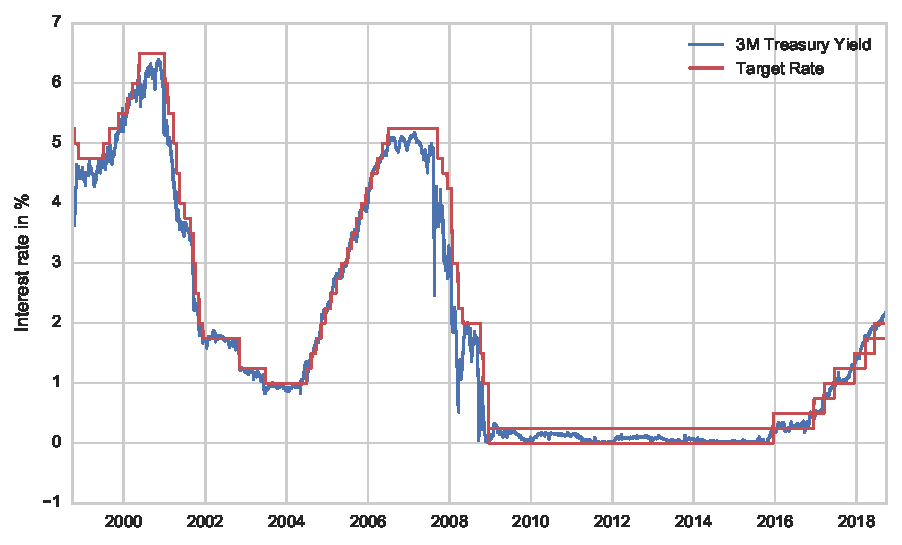
\includegraphics[scale=1]{Images/3Mtreasury.pdf}
%	\label{3Mtreasury}
%\end{figure}

The daily yield curve of the US Treasury bills, notes, and bonds for the period of October 1, 1998 to September 30, 2018 was retrieved from Thomson Reuters Datastream. Figure \ref{3Mtreasury} illustrates the development of the 3-month treasury yield as well as the target rate over the 20-year period. As explained in Chapter \ref{ExistingResearch}, \citeauthor{Ellingsen.2003} approximate unexpected monetary policy actions with the change in the 3-month T-bill rate. They argue, that the 3-month rate is sufficiently short to be determined by the target rate, but also sufficiently long to avoid noise from expectation errors \citep[~p. 13]{Ellingsen.2003}. Indeed, Figure \ref{3Mtreasury} shows that the 3-month T-bill rate and the target rate seem to move in tandem.  

The treasury yields for all other maturities are depicted in Figure \ref{alltreasury} in Appendix \ref{AppendixA}. Please note that for the 1-month rate the data series starts on July 31, 2001 and for the 7-year rate the series starts on May 26, 2009. Due to data availability, the 20-year rate is given as a constant maturity rate while the rates of the other maturities are given as bid yields. As expected, while the short term yields (up to 1 year) move quite closely with the target rate, the longer the maturity the more it emancipates itself from the target rate. 

%The bid yield is the yield figure that you get when you consider what your long-term return would be if you paid the bid price for the bond. 
%Bid yields are always higher than ask yields, because if the buyer were willing to take a yield that was equal to or less than the ask yield, then the seller would sell the bond to the buyer at that corresponding price. 
%Constant maturity is the theoretical value of a U.S. Treasury that is based on recent values of auctioned U.S. Treasuries. The value is obtained by the U.S. Treasury on a daily basis through interpolation of the Treasury yield curve which, in turn, is based on closing bid-yields of actively-traded Treasury securities. It is calculated using the daily yield curve of U.S. Treasury securities.

\begin{figure}
	\caption{Target rate and 3M treasury yield.}
	\centering
	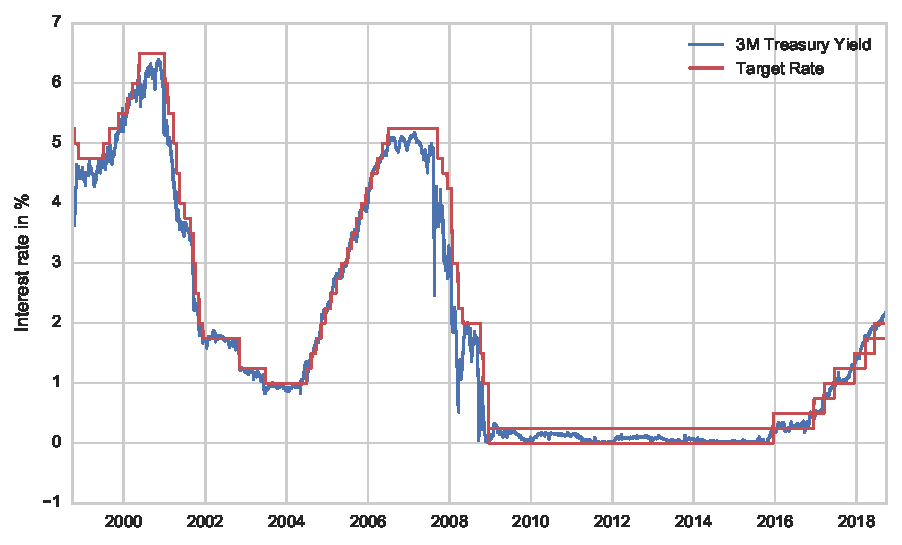
\includegraphics[scale=1]{Images/3Mtreasury.pdf}
	\label{3Mtreasury}
\end{figure}

\section{Text Data}

Articles are collected from the Dow Jones Factiva Database (https://global.factiva.com) by use of the search terms \textit{Federal Reserve} and \textit{interest rate}. Only articles that appeared in the \textit{United States} on the subject of \textit{interest rates} in a window of three days around each target rate adjustment (the day before, of, and after an adjustment as listed in Table \ref{tab:target}) are taken into account. The articles are mainly taken from the \textit{The Wall Street Journal}, \textit{Financial Times}, \textit{Reuters}, \textit{The Associated Press}, \textit{Market News International}, \textit{Dow Jones Institutional News}, \textit{Agence France}, and \textit{AFX}, as these newspapers seem to publish the most articles on the topic. 

From October 1, 1998 to September 30, 2018, 56 target rate adjustments have taken place, for which a total of 2'318 articles have been extracted. Since the FED changed its policy from undertaking a target rate change on the same day as a FOMC meeting to only doing so on the following day, articles $\pm1$ day around the official target rate change have been collected. This ensures that the articles capture any information, speculation, and interpretations that abound directly after the meeting, on the day of the target rate change as well as on the following day. On rare occasions, the number of articles ran in the several hundreds and only the most relevant have been selected. 

The final sample comprises between 14 and 97 publications for every policy day. In total, over $1'600'000$ tokens are extracted from these articles. After stop words have been removed, the token count drops to roughly $1'100'000$. (For more information on text preprocessing, see Chapter \ref{preprocessing}). Figure \ref{tokencount} in Appendix \ref{AppendixB} illustrates the spread of the text data across policy days and shows that the token count fluctuates quite drastically. More data is available for recent target rate adjustments, less for more historic adjustments.

Looking at the most common words in the entire text data base, as illustrated in Figure \ref{wcloud}, yields no surprises. As one might expect, the articles make heavy use of context specific vocabulary such as "interest rate", "federal reserve", "economy", but also of terms appropriate for a financial environment such as "basis point", "percentage point", or "investor". Even just considering the titles of the articles yields an almost identical word distribution. Thus, headlines appear to be just as factual and technical as the general text body. Overall, this is a first indication that while there is a set vocabulary to talk about the facts of a target rate change, there is no similarly systematic vocabulary to express interpretations and sentiments surrounding such a change. 

\begin{figure}
	\caption{Wordcloud illustrating the most common words across all articles.}
	\centering
	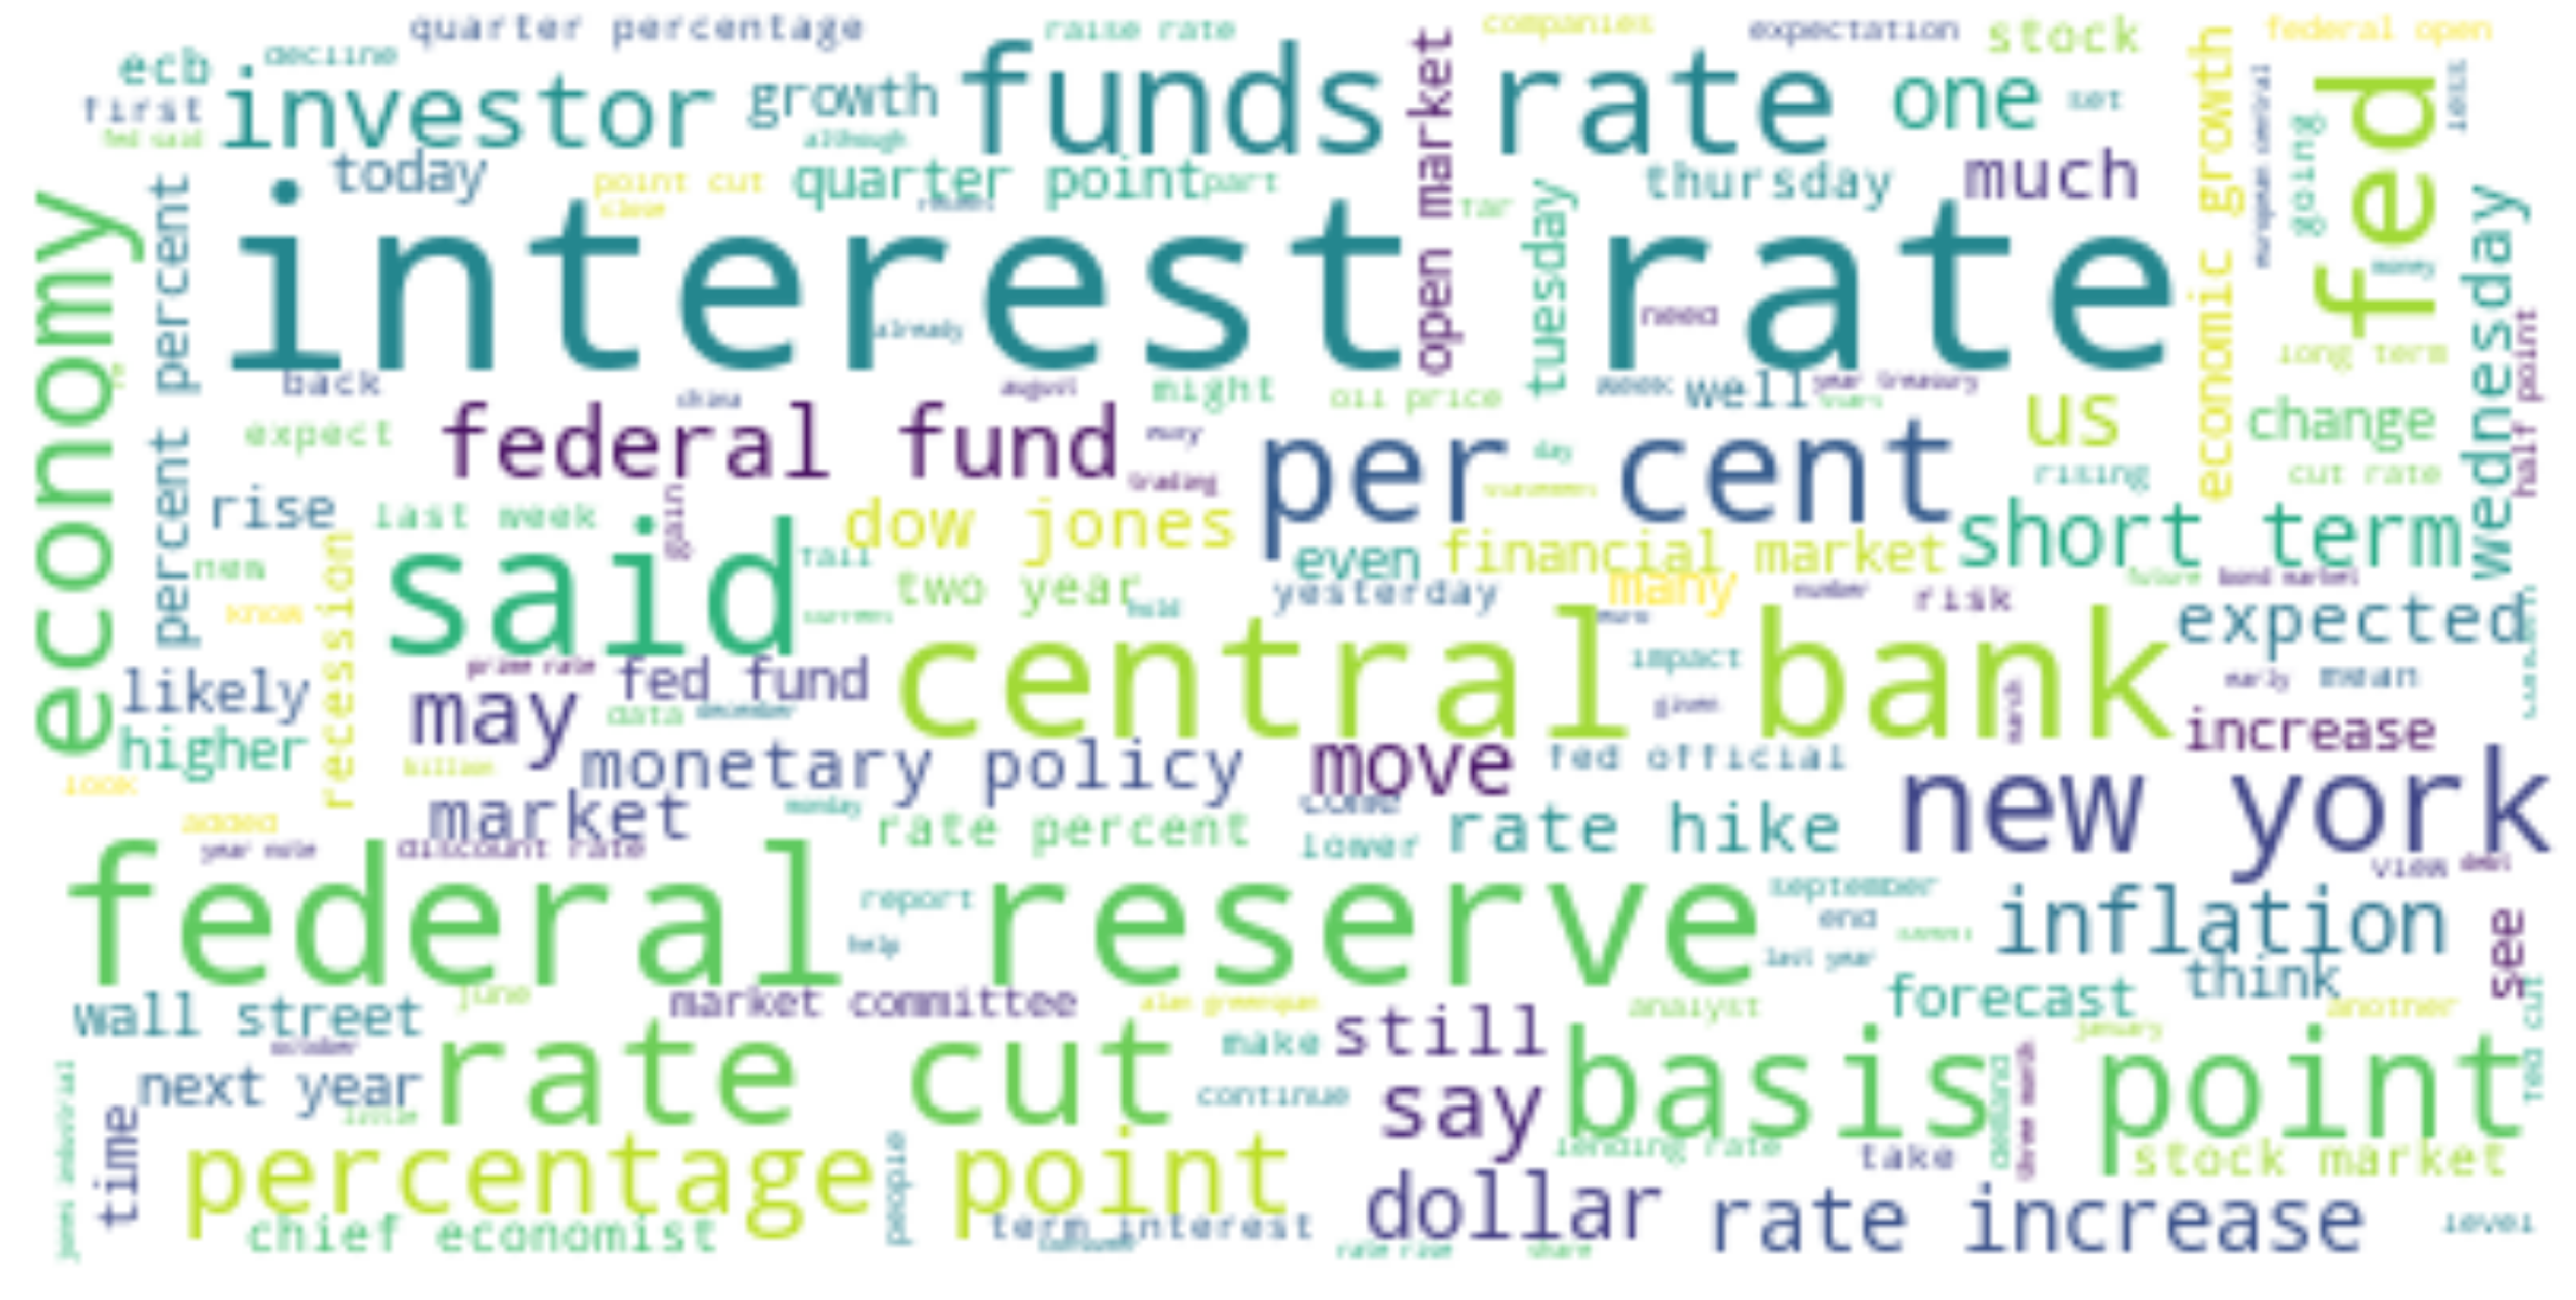
\includegraphics[scale=0.2]{Images/wordcloud.pdf}
	\label{wcloud}
\end{figure}


	
%More than 100 articles, needed selection: 15.12.2016 / 17.12.2015 / 22.01.2008 / 18.09.2007/ // 08.10.2008 corrupted file! - no wall street journal//


\section{Methodology}


\subsection{Text Preprocessing}\label{preprocessing}
For almost all purposes of computational linguistics, the texts have to be processed and prepared. To that end, text data first needs to be segmented into words, that is the sequence of characters that make up a text needs to be broken down to locate the word boundaries. Words identified thus are referred to as tokens and the process is known as tokenization \cite[p. 10]{Palmer.2010}. I apply the word tokenizer of the nltk package \citep{Bird.2010}, as this application is prepared to deal with frequently occurring character sequences appertaining to the English language, such as contractions. \citet[pp. 16-19]{Palmer.2010} rightly points out that there exists plenty of tokenization ambiguity, even in a language where the words are generally space-delimited. Some of this ambiguity is hard to resolve, such as the use of apostrophes for the genitive form of a noun, for the plural form, and for verbal contractions. \textcolor{red}{Could give a (code) example in the appendix}

In a next step, frequent words that carry little information, commonly referred to as stop words, are removed from the text. 

In a next step, Porter stemmer 

 especially concerning punctuation,  already needs to address the ambiguity that is inherent in natural language. there is a lot of ambiguity in natrual language that 

Depending on what we need for further processing, the text needs to be prepared 
In a first step, the text data must be prepared for analysis. To that end, the text is split into meaningful tokens. I used my own tokenizer for this task,
Porter stemmer,  
Preprocessing of text:
 - tokenization, how and which one chosen and why?
 - stemmer 
 	-stop word removal
 	- nltk.tokenize.mwe module
 	
%[word_tokenize(t) for t in sent_tokenize(s)]
%[['Good', 'muffins', 'cost', '\$', '3.88', 'in', 'New', 'York', '.'],
%['Please', 'buy', 'me', 'two', 'of', 'them', '.'], ['Thanks', '.']]



\section{NOTES}
Besprechung - 24.09.2018
------------------------

- Frage Juan Pablo Ortega ob er Korreferent sein will
- nur zwei Narrative finden, ohne Daten vorgeben (Texte nach Meeting verwenden, weil sonst ja nicht Interpretation gefunden wird), dann schauen geht die Kurve beim einten Narrativ hoch beim anderen runter
- es sollten auch die non-target rate sdjustments verwendet werden, weil ansonsten j schon eine Selektion stattfindet - ABER: stimmt das wirklich, weil wenn kein adjustment, dann bewegt sich doch die Kurve nur gemäss neue Infos auf dem Markt, - also vielleicht doch besser keine adjustment heisst non-policy day?

- Example: nach nine eleven gab es tatsächlich ein paar unangemeldetet meetings und daher komische effekte weil wirklich überraschende Verschiebungen in der interest rate

- modell ist gut, unsupervised learning verwenden, nicht vorher sagen, wo geht's hoch und wo runter, und dann ev. auch out-of sample probieren, aber das wäre Paradedisplizin, keine Garantie, dass das funktoniert

---my thoughts before meeting

all absolute Fed target rate changes during the sample period -- ev. sind 10 Jahre nicht genug, vor allem weil es dann nur die extraordinary years sind - 20 Jahre? training and testing samples? aber dann müsste man annehmen, dass die Narrative über die Jahre gleichbleiben? oder aber man nimmt einzelne Datenpunkte aus dem sample raus? einzelne Tage (wohl zu wenige Observations) - einzelne ARtikel - sagt das was aus?


\chapter{Results}

\chapter{Conclusion}


\newpage

\phantomsection 
\addcontentsline{toc}{chapter}{References} 
%\renewcommand\bibname{References}

\bibliography{EconomicNarrative}



\newpage

\appendix
\noappendicestocpagenum
\addappheadtotoc
%%\appendixpage



\renewcommand{\theequation}{A.\arabic{equation}}


\chapter{Target Rate and Yield Curves}\label{AppendixA}
\vspace{-0.5cm}
%\lipsum[2-4]

\begin{table}[h] % Add the following just after the closing bracket on this line to specify a position for the table on the page: [h], [t], [b] or [p] - these mean: here, top, bottom and on a separate page, respectively
	\centering % Centres the table on the page, comment out to left-justify
	\begin{tabular}{r r r r r r r } % The final bracket specifies the number of columns in the table along with left and right borders which are specified using vertical pipes (|); each column can be left, right or center-justified using l, r or c. Columns will widen to hold the content in them by default, to specify a precise width, use p{width}, e.g. p{5cm}
		\toprule % Top horizontal line
%		& & & & & \multicolumn{2}{l}{FOMC Meeting on} & & & & & & \multicolumn{2}{l}{FOMC Meeting on} \\ % Amalgamating several columns into one cell is done using the \multicolumn command with the number of columns to amalgamate as the first argument and then the justification (l, r or c)
		%		\cmidrule(l){6-7} % Horizontal line spanning less than the full width of the table - you can add (r) or (l) just before the opening curly bracket to shorten the rule on the left or right side
%		Date & $Tgt_{low}$ & $Tgt_{up}$ & $\Delta Tgt_{low}$ & $\Delta Tgt_{up}$ & day prior &  same day & Date & $Tgt_{low}$ & $Tgt_{up}$ & $\Delta Tgt_{low}$ & $\Delta Tgt_{up}$ & day prior &  same day \\ % Column names row
		\multicolumn{7}{c}{Dates of all FOMC meetings since January 1, 1998} \\
		\midrule % In-table horizontal line
						26.09.2018 & 18.03.2015 & 13.12.2011 & *07.02.2009 & 12.12.2006 & 12.08.2003 & 31.01.2001 \\
						01.08.2018 & 28.01.2015 & *28.11.2011 & 28.01.2009 & 25.10.2006 & 25.06.2003 & *03.01.2001 \\
						13.06.2018 & 17.12.2014 & 02.11.2011 & *16.01.2009 & 20.09.2006 & 06.05.2003 & 19.12.2000 \\
						02.05.2018 & 29.10.2014 & 21.09.2011 & 16.12.2008 & 08.08.2006 & *16.04.2003 & 15.11.2000 \\
						21.03.2018 & 17.09.2014 & 09.08.2011 & 29.10.2008 & 29.06.2006 & *08.04.2003 & 03.10.2000 \\
						31.01.2018 & 30.07.2014 & *01.08.2011 & *07.10.2008 & 10.05.2006 & *01.04.2003 & 22.08.2000 \\
						13.12.2017 & 18.06.2014 & 22.06.2011 & *29.09.2008 & 28.03.2006 & *25.03.2003 & 28.06.2000 \\
						01.11.2017 & 30.04.2014 & 27.04.2011 & 16.09.2008 & 31.01.2006 & 18.03.2003 & 16.05.2000 \\
						20.09.2017 & 19.03.2014 & 15.03.2011 & 05.08.2008 & 13.12.2005 & 29.01.2003 & 21.03.2000 \\
						26.07.2017 & *04.03.2014 & 26.01.2011 & *24.07.2008 & 01.11.2005 & 10.12.2002 & 02.02.2000 \\
						14.06.2017 & 29.01.2014 & 14.12.2010 & 25.06.2008 & 20.09.2005 & 06.11.2002 & 21.12.1999 \\
						03.05.2017 & 18.12.2013 & 03.11.2010 & 30.04.2008 & 09.08.2005 & 24.09.2002 & 16.11.1999 \\
						15.03.2017 & 30.10.2013 & *15.10.2010 & 18.03.2008 & 30.06.2005 & 13.08.2002 & 05.10.1999 \\
						01.02.2017 & *16.10.2013 & 21.09.2010 & *10.03.2008 & 03.05.2005 & 26.06.2002 & 24.08.1999 \\
						14.12.2016 & 18.09.2013 & 10.08.2010 & 30.01.2008 & 22.03.2005 & 07.05.2002 & 30.06.1999 \\
						02.11.2016 & 31.07.2013 & 23.06.2010 & *21.01.2008 & 02.02.2005 & 19.03.2002 & 18.05.1999 \\
						21.09.2016 & 19.06.2013 & *09.05.2010 & *09.01.2008 & 14.12.2004 & 30.01.2002 & 30.03.1999 \\
						27.07.2016 & 01.05.2013 & 28.04.2010 & 11.12.2007 & 10.11.2004 & 11.12.2001 & 03.02.1999 \\
						15.06.2016 & 20.03.2013 & 16.03.2010 & *06.12.2007 & 21.09.2004 & 06.11.2001 & 22.12.1998 \\
						27.04.2016 & 30.01.2013 & 27.01.2010 & 31.10.2007 & 10.08.2004 & 02.10.2001 & 17.11.1998 \\
						16.03.2016 & 12.12.2012 & 16.12.2009 & 18.09.2007 & 30.06.2004 & *17.09.2001 & *15.10.1998 \\
						27.01.2016 & 24.10.2012 & 04.11.2009 & *16.08.2007 & 04.05.2004 & *13.09.2001 & 29.09.1998 \\
						16.12.2015 & 13.09.2012 & 23.09.2009 & *10.08.2007 & 16.03.2004 & 21.08.2001 & *21.09.1998 \\
						28.10.2015 & 01.08.2012 & 12.08.2009 & 07.08.2007 & 28.01.2004 & 27.06.2001 & 18.08.1998 \\
						17.09.2015 & 20.06.2012 & 24.06.2009 & 28.06.2007 & 09.12.2003 & 15.05.2001 & 01.07.1998 \\
						29.07.2015 & 25.04.2012 & *03.06.2009 & 09.05.2007 & 28.10.2003 & *18.04.2001 & 19.05.1998 \\
						17.06.2015 & 13.03.2012 & 29.04.2009 & 21.03.2007 & 16.09.2003 & *11.04.2001 & 31.03.1998 \\
						29.04.2015 & 25.01.2012 & 18.03.2009 & 31.01.2007 &  & 20.03.2001 & 04.02.1998 \\
						\midrule																
						\multicolumn{6}{l}{* indicates an unscheduled meeting/conference call} & \\
		%		\midrule % In-table horizontal line
		%		Average Rate & 0.920 & 0.882 & 0.477 & 0.539 & 0.923\\ % Summary/total row
		\bottomrule % Bottom horizontal line
	\end{tabular}
	\caption{FOMC meetings.} % Table caption, can be commented out if no caption is required
	\label{tab:meetings} % A label for referencing this table elsewhere, references are used in text as \ref{label}
\end{table}




\newpage
\thispagestyle{empty}

\begin{sidewaystable} % Add the following just after the closing bracket on this line to specify a position for the table on the page: [h], [t], [b] or [p] - these mean: here, top, bottom and on a separate page, respectively
	\centering % Centres the table on the page, comment out to left-justify
	\begin{tabular}{r r r r r c c | r r r r r c c } % The final bracket specifies the number of columns in the table along with left and right borders which are specified using vertical pipes (|); each column can be left, right or center-justified using l, r or c. Columns will widen to hold the content in them by default, to specify a precise width, use p{width}, e.g. p{5cm}
		\toprule % Top horizontal line
		& & & & & \multicolumn{2}{l}{FOMC Meeting on} & & & & & & \multicolumn{2}{l}{FOMC Meeting on} \\ % Amalgamating several columns into one cell is done using the \multicolumn command with the number of columns to amalgamate as the first argument and then the justification (l, r or c)
		%		\cmidrule(l){6-7} % Horizontal line spanning less than the full width of the table - you can add (r) or (l) just before the opening curly bracket to shorten the rule on the left or right side
		Date & $Tgt_{low}$ & $Tgt_{up}$ & $\Delta Tgt_{low}$ & $\Delta Tgt_{up}$ & day prior &  same day & Date & $Tgt_{low}$ & $Tgt_{up}$ & $\Delta Tgt_{low}$ & $\Delta Tgt_{up}$ & day prior &  same day \\ % Column names row
		\midrule % In-table horizontal line
		27.09.2018 & 2.00\% & 2.25\% & 25  &  -   & 1 & 0 & 14.12.2004 & 2.25\% &  - & 25  &  - & 0 & 1 \\
		14.06.2018 & 1.75\% & 2.00\% & 25  &  -   & 1 & 0 & 10.11.2004 & 2.00\% &  - & 25  &  - & 0 & 1 \\
		22.03.2018 & 1.50\% & 1.75\% & 25  &  -   & 1 & 0 & 21.09.2004 & 1.75\% &  - & 25  &  - & 0 & 1 \\
		14.12.2017 & 1.25\% & 1.50\% & 25  &  -   & 1 & 0 & 10.08.2004 & 1.50\% &  - & 25  &  - & 0 & 1 \\
		15.06.2017 & 1.00\% & 1.25\% & 25  &  -   & 1 & 0 & 30.06.2004 & 1.25\% &  - & 25  &  - & 0 & 1 \\
		16.03.2017 & 0.75\% & 1.00\% & 25  &  -   & 1 & 0 & \cellcolor{lightgray!25}25.06.2003 & \cellcolor{lightgray!25}1.00\% &  \cellcolor{lightgray!25}- & \cellcolor{lightgray!25}-25 &  \cellcolor{lightgray!25}- & 0 & 1 \\
		15.12.2016 & 0.50\% & 0.75\% & 25  &  -   & 1 & 0 & \cellcolor{lightgray!25}06.11.2002 & \cellcolor{lightgray!25}1.25\% &  \cellcolor{lightgray!25}- & \cellcolor{lightgray!25}-50 &  \cellcolor{lightgray!25}- & 0 & 1 \\
		17.12.2015 & 0.25\% & 0.50\% & 25  &  -   & 1 & 0 & \cellcolor{lightgray!25}11.12.2001 & \cellcolor{lightgray!25}1.75\% &  \cellcolor{lightgray!25}- & \cellcolor{lightgray!25}-25 &  \cellcolor{lightgray!25}- & 0 & 1 \\
		\cellcolor{lightgray!25}16.12.2008 & \cellcolor{lightgray!25}0.00\% & \cellcolor{lightgray!25}0.25\% & \cellcolor{lightgray!25}-75 & \cellcolor{lightgray!25}-100 & 0 & 1 & \cellcolor{lightgray!25}06.11.2001 & \cellcolor{lightgray!25}2.00\% &  \cellcolor{lightgray!25}- & \cellcolor{lightgray!25}-50 &  \cellcolor{lightgray!25}- & 0 & 1 \\
		\cellcolor{lightgray!25}29.10.2008 & \cellcolor{lightgray!25}1.00\% &   \cellcolor{lightgray!25}-    & \cellcolor{lightgray!25}-50 &  \cellcolor{lightgray!25}-   & 0 & 1 & \cellcolor{lightgray!25}02.10.2001 & \cellcolor{lightgray!25}2.50\% &  \cellcolor{lightgray!25}- & \cellcolor{lightgray!25}-50 &  \cellcolor{lightgray!25}- & 0 & 1 \\
		\cellcolor{lightgray!25}*08.10.2008 & \cellcolor{lightgray!25}1.50\% &  \cellcolor{lightgray!25} -    & \cellcolor{lightgray!25}-50 &  \cellcolor{lightgray!25}-   & 1 & 0 & \cellcolor{lightgray!25}*17.09.2001 & \cellcolor{lightgray!25}3.00\% &  \cellcolor{lightgray!25}- & \cellcolor{lightgray!25}-50 &  \cellcolor{lightgray!25}- & 0 & 1 \\
		\cellcolor{lightgray!25}30.04.2008 & \cellcolor{lightgray!25}2.00\% &  \cellcolor{lightgray!25} -    & \cellcolor{lightgray!25}-25 &  \cellcolor{lightgray!25}-   & 0 & 1 & \cellcolor{lightgray!25}21.08.2001 & \cellcolor{lightgray!25}3.50\% &  \cellcolor{lightgray!25}- & \cellcolor{lightgray!25}-25 &  \cellcolor{lightgray!25}- & 0 & 1 \\
		\cellcolor{lightgray!25}18.03.2008 & \cellcolor{lightgray!25}2.25\% &  \cellcolor{lightgray!25} -    & \cellcolor{lightgray!25}-75 &  \cellcolor{lightgray!25}-   & 0 & 1 & \cellcolor{lightgray!25}27.06.2001 & \cellcolor{lightgray!25}3.75\% &  \cellcolor{lightgray!25}- & \cellcolor{lightgray!25}-25 &  \cellcolor{lightgray!25}- & 0 & 1 \\
		\cellcolor{lightgray!25}30.01.2008 & \cellcolor{lightgray!25}3.00\% &  \cellcolor{lightgray!25} -    & \cellcolor{lightgray!25}-50 &  \cellcolor{lightgray!25}-   & 0 & 1 & \cellcolor{lightgray!25}15.05.2001 & \cellcolor{lightgray!25}4.00\% &  \cellcolor{lightgray!25}- & \cellcolor{lightgray!25}-50 &  \cellcolor{lightgray!25}- & 0 & 1 \\
		\cellcolor{lightgray!25}*22.01.2008 & \cellcolor{lightgray!25}3.50\% &  \cellcolor{lightgray!25} -    & \cellcolor{lightgray!25}-75 &  \cellcolor{lightgray!25}-   & 1 & 0 & \cellcolor{lightgray!25}*18.04.2001 & \cellcolor{lightgray!25}4.50\% &  \cellcolor{lightgray!25}- & \cellcolor{lightgray!25}-50 &  \cellcolor{lightgray!25}- & 0 & 1 \\
		\cellcolor{lightgray!25}11.12.2007 & \cellcolor{lightgray!25}4.25\% &  \cellcolor{lightgray!25} -    & \cellcolor{lightgray!25}-25 &  \cellcolor{lightgray!25}-   & 0 & 1 & \cellcolor{lightgray!25}20.03.2001 & \cellcolor{lightgray!25}5.00\% &  \cellcolor{lightgray!25}- & \cellcolor{lightgray!25}-50 &  \cellcolor{lightgray!25}- & 0 & 1 \\
		\cellcolor{lightgray!25}31.10.2007 & \cellcolor{lightgray!25}4.50\% &  \cellcolor{lightgray!25} -    & \cellcolor{lightgray!25}-25 &  \cellcolor{lightgray!25}-   & 0 & 1 & \cellcolor{lightgray!25}31.01.2001 & \cellcolor{lightgray!25}5.50\% &  \cellcolor{lightgray!25}- & \cellcolor{lightgray!25}-50 &  \cellcolor{lightgray!25}- & 0 & 1 \\
		\cellcolor{lightgray!25}18.09.2007 & \cellcolor{lightgray!25}4.75\% &  \cellcolor{lightgray!25} -    & \cellcolor{lightgray!25}-50 &  \cellcolor{lightgray!25}-   & 0 & 1 & \cellcolor{lightgray!25}*03.01.2001 & \cellcolor{lightgray!25}6.00\% &  \cellcolor{lightgray!25}- & \cellcolor{lightgray!25}-50 &  \cellcolor{lightgray!25}- & 0 & 1 \\
		29.06.2006 & 5.25\% &   -    & 25  &  -   & 0 & 1 & 16.05.2000 & 6.50\% &  - & 50  &  - & 0 & 1 \\
		10.05.2006 & 5.00\% &   -    & 25  &  -   & 0 & 1 & 21.03.2000 & 6.00\% &  - & 25  &  - & 0 & 1 \\
		28.03.2006 & 4.75\% &   -    & 25  &  -   & 0 & 1 & 02.02.2000 & 5.75\% &  - & 25  &  - & 0 & 1 \\
		31.01.2006 & 4.50\% &   -    & 25  &  -   & 0 & 1 & 16.11.1999 & 5.50\% &  - & 25  &  - & 0 & 1 \\
		13.12.2005 & 4.25\% &   -    & 25  &  -   & 0 & 1 & 24.08.1999 & 5.25\% &  - & 25  &  - & 0 & 1 \\
		01.11.2005 & 4.00\% &   -    & 25  &  -   & 0 & 1 & 30.06.1999 & 5.00\% &  - & 25  &  - & 0 & 1 \\
		20.09.2005 & 3.75\% &   -    & 25  &  -   & 0 & 1 & \cellcolor{lightgray!25}17.11.1998 & \cellcolor{lightgray!25}4.75\% &  \cellcolor{lightgray!25}- & \cellcolor{lightgray!25}-25 &  \cellcolor{lightgray!25}- & 0 & 1 \\
		09.08.2005 & 3.50\% &   -    & 25  &  -   & 0 & 1 & \cellcolor{lightgray!25}*15.10.1998 & \cellcolor{lightgray!25}5.00\% &  \cellcolor{lightgray!25}- & \cellcolor{lightgray!25}-25 &  \cellcolor{lightgray!25}- & 0 & 1 \\
		30.06.2005 & 3.25\% &   -    & 25  &  -   & 0 & 1 & \cellcolor{lightgray!25}29.09.1998 & \cellcolor{lightgray!25}5.25\% &  \cellcolor{lightgray!25}- & \cellcolor{lightgray!25}-25 &  \cellcolor{lightgray!25}- & 0 & 1 \\
		03.05.2005 & 3.00\% &   -    & 25  &  -   & 0 & 1 &            &      &  &     &  &   &   \\
		22.03.2005 & 2.75\% &   -    & 25  &  -   & 0 & 1 &            &      &  &     &  &   &   \\
		02.02.2005 & 2.50\% &   -    & 25  &  -   & 0 & 1 &            &      &  &     &  &   & \\	
		\midrule																
		\multicolumn{13}{l}{ $\Delta Tgt$ are given in basis points \hspace{1cm}  * indicates a target rate adjustment following an unscheduled meeting} & \\
		%		\midrule % In-table horizontal line
		%		\midrule % In-table horizontal line
		%		Average Rate & 0.920 & 0.882 & 0.477 & 0.539 & 0.923\\ % Summary/total row
		\bottomrule % Bottom horizontal line
	\end{tabular}
	\caption{Target rate adjustments since January 1, 1998.} % Table caption, can be commented out if no caption is required
	\label{tab:target} % A label for referencing this table elsewhere, references are used in text as \ref{label}
\end{sidewaystable}

\newpage
\thispagestyle{firststyle}

\begin{figure}
	\caption{Target rate and treasury yields of all maturities.}
	\centering
	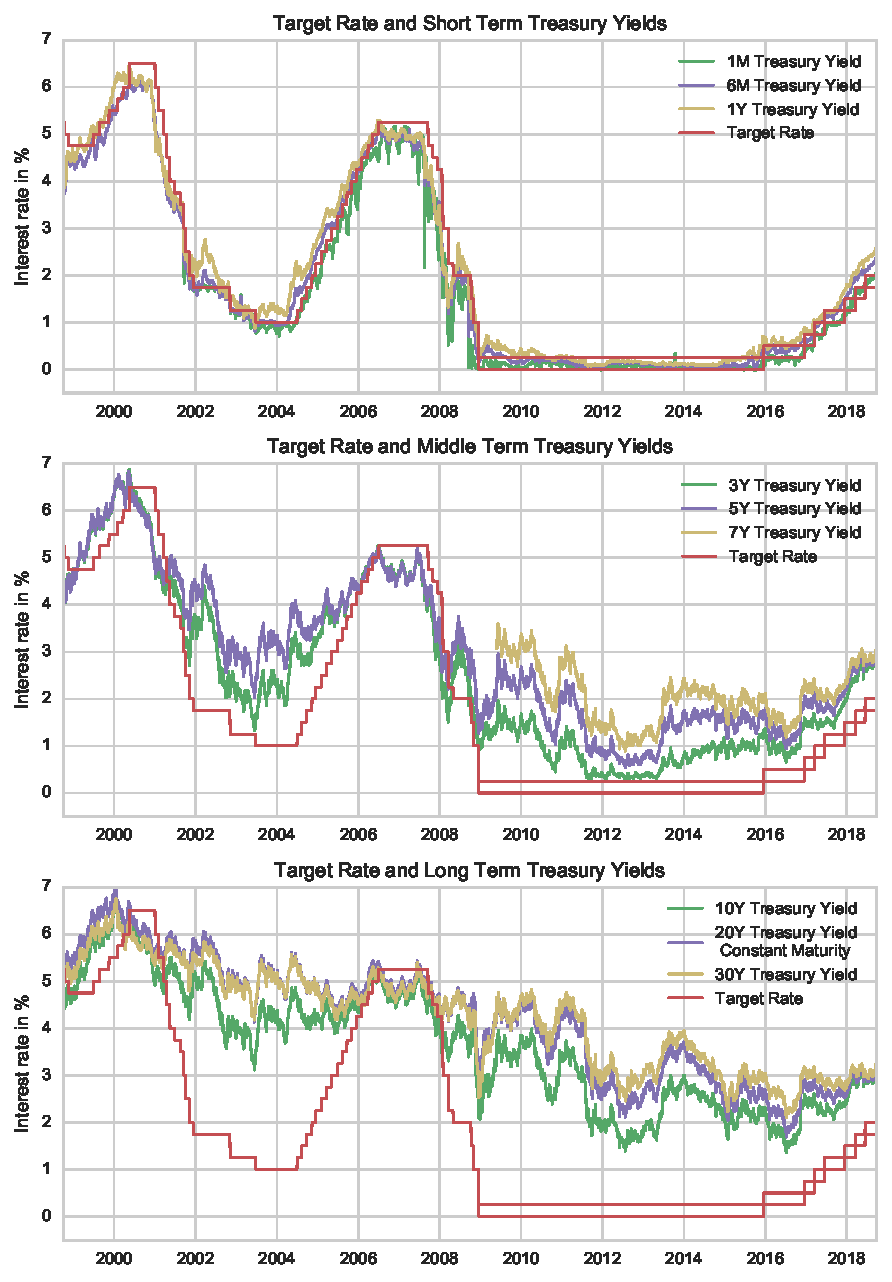
\includegraphics[scale=1]{Images/alltreasury.pdf}
	\label{alltreasury}
\end{figure}


\renewcommand{\theequation}{B.\arabic{equation}}


\chapter{Text data}\label{AppendixB}

\begin{figure}
	\caption{Token and article count for every policy day.}
	\centering
	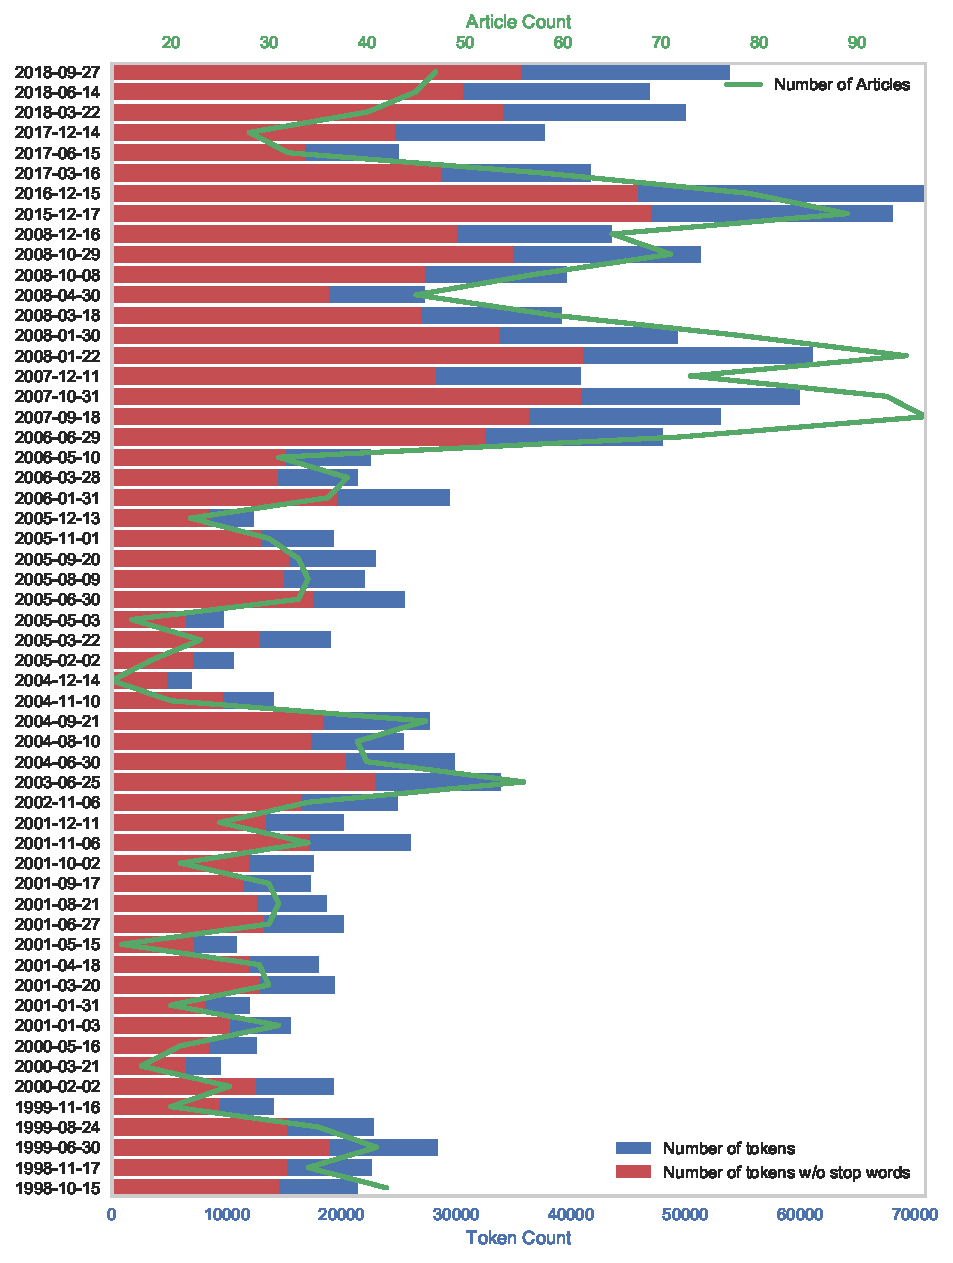
\includegraphics[scale=1]{Images/tokencount.pdf}
	\label{tokencount}
\end{figure}



\renewcommand{\theequation}{C.\arabic{equation}}


\chapter{Whatever may come...}



\section{For Example... }

\lipsum[2-8]

\newpage
{\pagestyle{firststyle}
	
\chapter*{Declaration of Authorship}

"I hereby declare
\begin{itemize}
	\item that I have written this thesis without any help from others and without the use of
	documents and aids other than those stated above;
	\item that I have mentioned all the sources used and that I have cited them correctly
	according to established academic citation rules;
	\item that I have acquired any immaterial rights to materials I may have used such as images
	or graphs, or that I have produced such materials myself;
	\item that the topic or parts of it are not already the object of any work or examination of
	another course unless this has been explicitly agreed on with the faculty member in
	advance and is referred to in the thesis;
	\item that I will not pass on copies of this work to third parties or publish them without the
	University’s written consent if a direct connection can be established with the
	University of St.Gallen or its faculty members;
	\item that I am aware that my work can be electronically checked for plagiarism and that I
	hereby grant the University of St.Gallen copyright in accordance with the Examination
	Regulations in so far as this is required for administrative action;
	\item that I am aware that the University will prosecute any infringement of this declaration
	of authorship and, in particular, the employment of a ghostwriter, and that any such
	infringement may result in disciplinary and criminal consequences which may result
	in my expulsion from the University or my being stripped of my degree."
\end{itemize}

%\noindent By submitting this academic term paper, I confirm through my conclusive action that I am
%submitting the Declaration of Authorship, that I have read and understood it, and that it is
%true.

%\hrule
\vspace*{3cm}
%\hrule


\dotbox{Location, Date} \hfill \dotbox{Signature}\\

\vspace*{.5 cm}
\noindent By submitting this academic term paper, I confirm through my conclusive action that I am
submitting the Declaration of Authorship, that I have read and understood it, and that it is
true.
\cleardoublepage
}
\end{document}
